\section{Methodologies}
\label{methods}

\subsection{Sentiment Analysis}
\subsubsection{Data Preprocessing}
For conducting the sentiment analysis, preprocessing of the data was necessary. Since the 65,393 speeches contained in the corpus were provided as separate text files, we decided to combine the speeches for each year, allowing for an analysis of the sentiment development over time. 
We resolved several issues that arose in the process, e.g. duplicate speech IDs or missing meta data. 

The yearly overview used for the analysis included the speech ID, date, speech text, cleaned text, topic, country, name of the speaker, participant type, subjectivity score, sentiment score, number of positive sentences, and number of negative sentences for each speech.

In order to perform inter- and intracountry comparisons, we calculated the yearly average for each feature (i.e. sentiment, subjectivity, positive and negative sentences) for each country. Using this average data, we also calculated the standard deviation of the scores for each country over time. 

We also created additional overviews for analyzing the the core nations of the UNSC, the sentiment of the core nations related to the Iraq War. Lastly, we created two more overviews for a detailed country-level sentiment analysis during two specific resolutions related to the invasion of Iraq. 

After creating these data overviews in Python, we stored each one locally as \texttt{csv} file since computation on each access of the data would have been too costly. For the purpose of easy access, we prepared several helper functions which load the data into the Python data structure \texttt{Pandas DataFrame}. We chose the DataFrame for data storage and manipulation since it efficiently handles large data and is much more flexible than standard data structures.

\subsubsection{Sentiment Polarity and Subjectivity}

As mentioned in section 2.2.1, we relied on commonly used automatic sentiment analysis tools for our analysis.  As for the processing of the speeches for this analysis, we chose to clean the speeches, which means that we removed stop words (common words with no inherent meaning) and transformed the text into lowercase. This was done for the sentiment analysis using VADER and the subjectivity analysis using TextBlob. For the calculation of the amount of positive and negative sentences per speech with AFINN, we also tokenized the words in the speeches. Tokenization yielded no improved results for sentiment and subjectivity analysis. For text manipulation, we used the Python \texttt{nltk} library.

As for the visualizations of the analysis results, we relied on Python's \texttt{matplotlib} plotting library, expanded with the \texttt{Seaborn} library. All analyses and data handling was performed with \texttt{Python 3.7.4}.  Our final product for sentiment analysis is a human-readable \texttt{json} file mapping UNSC speech IDs to sentiment and subjectivity scores, available in our public GitHub repository\footnote{https://github.com/atreyasha/sentiment-argument-mining}.

\subsection{Argumentation Mining}
\subsubsection{US Election Debate Corpus}
\label{used}

\begin{figure}[b!]
    \centering
    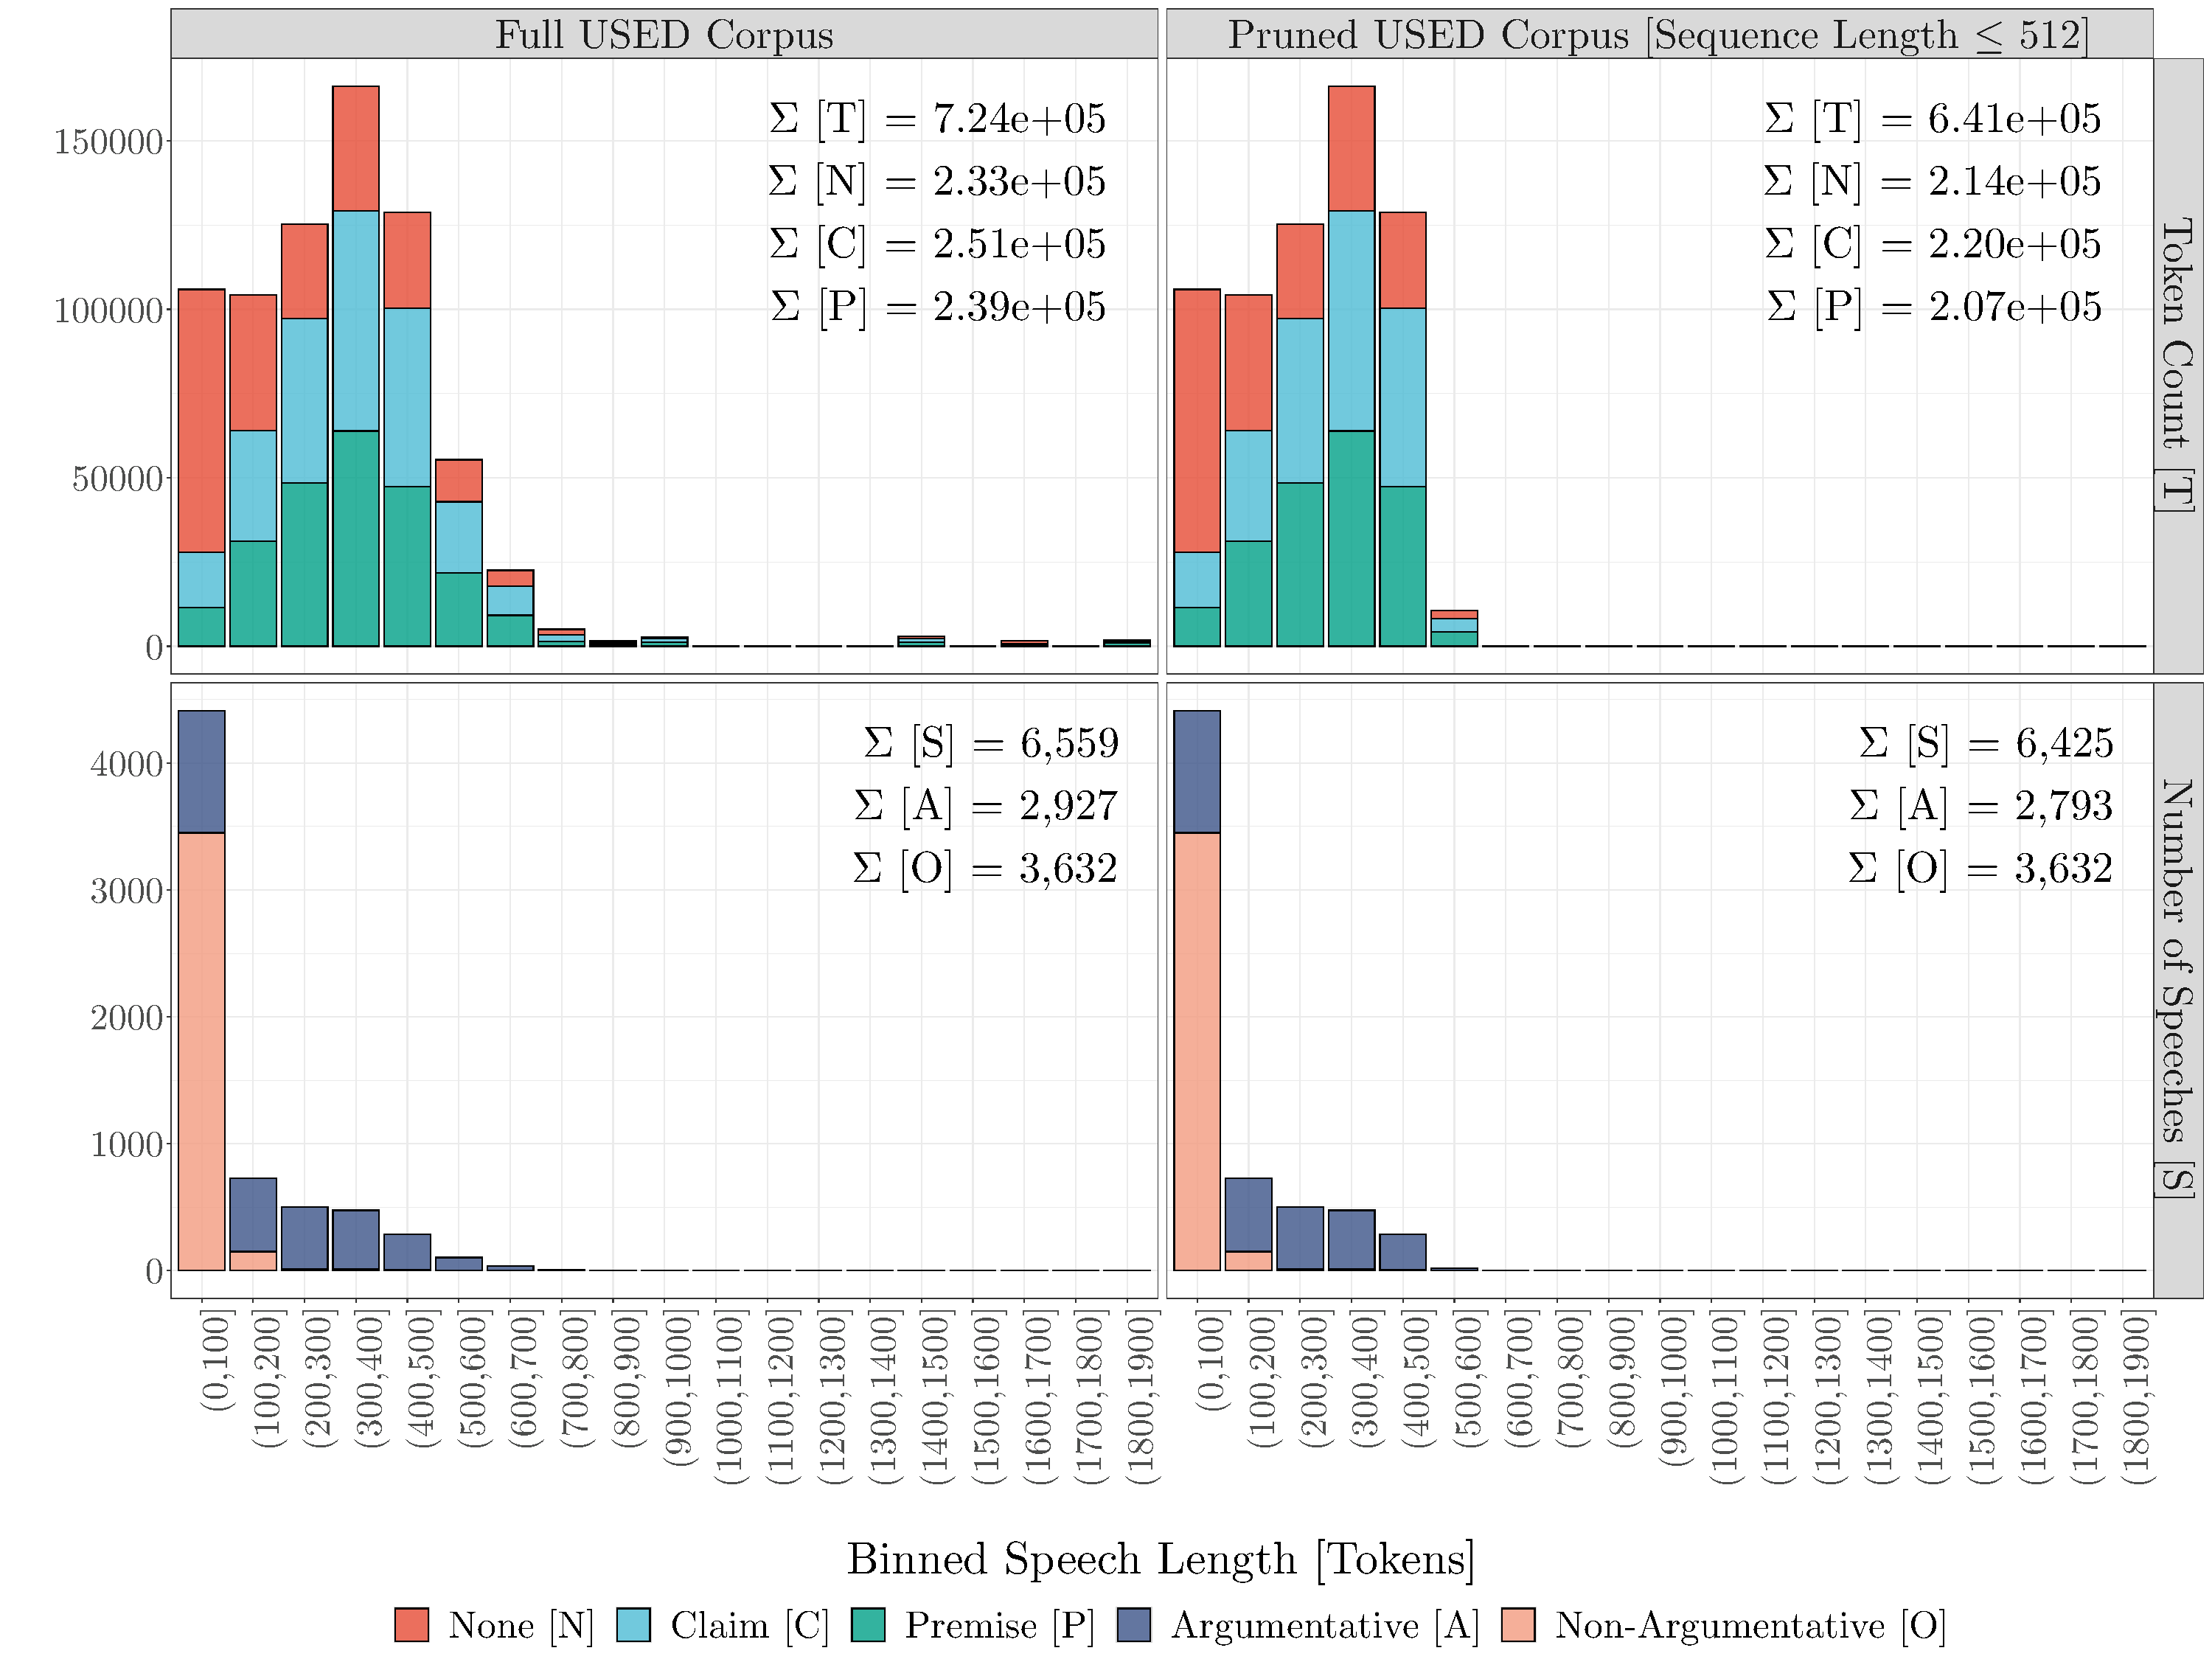
\includegraphics[trim={1.0cm 0cm 0cm 0cm},clip,width=\textwidth]{img/token_dist_US_length_combined.pdf}
    \caption{Full USED corpus (left-column) and pruned USED corpus (right-column) by binned speech length with token count (top-row) and number of speeches (bottom-row)}
    \label{used_distribution_combined}
\end{figure}

As mentioned in section \ref{corpora}, we decided that the USED corpus would be the best choice for us to train an argumentation classifier. Regarding corpus-specific ADUs, \citet{haddadan-etal-2019-yes}, the authors of the USED corpus, define a claim (in the political domain) as \textit{``a policy advocated by a party or a candidate to be undertaken which needs to be justified in order to be accepted by the audience."} Similarly, they define a premise as an \textit{``assertion made by the debaters for supporting their claims (i.e., reasons or justifications)."}

The USED corpus is annotated at a character-span level, with spans being annotated either as claims or premises. It follows naturally that character spans that are not annotated can be considered as non-argumentative text. Furthermore, the USED corpus also has been annotated for linkages between argumentative spans. This typically comes in the form of $N$ consecutive premises being recorded after a claim; which indicate that those $N$ premises belong to the preceding claim. Linkage types, such as attack or support relations, are not annotated in this corpus.

As mentioned in section \ref{models}, we would like to conduct argumentation mining using a bottom-up approach by using sequence tagging; since this process would also lend itself to quick application on the UNSC corpus. Given the time and resource restrictions in this study, we decided to focus solely on classifying tokens into argumentation candidates; such as claims, premises or neither. We omit the task of linking spans from claims and premises and instead recommend this task for further studies.

It is also worth noting that \citet{haddadan-etal-2019-yes} performed a similar task as ours on the USED corpus. However, they trained a classifier to identify argumentative sentences and argumentative sentence types. Performing such a task at a sentence-level removes many of the fine-grained character spans which do not necessarily span entire sentences. In fact, multiple character spans can be included within a sentence. As a result, we will be unable to compare our results directly with theirs since we perform a more fine-grained token-level classification task.

\subsubsection{Data Preprocessing}

\begin{figure}[b!]
    \centering
    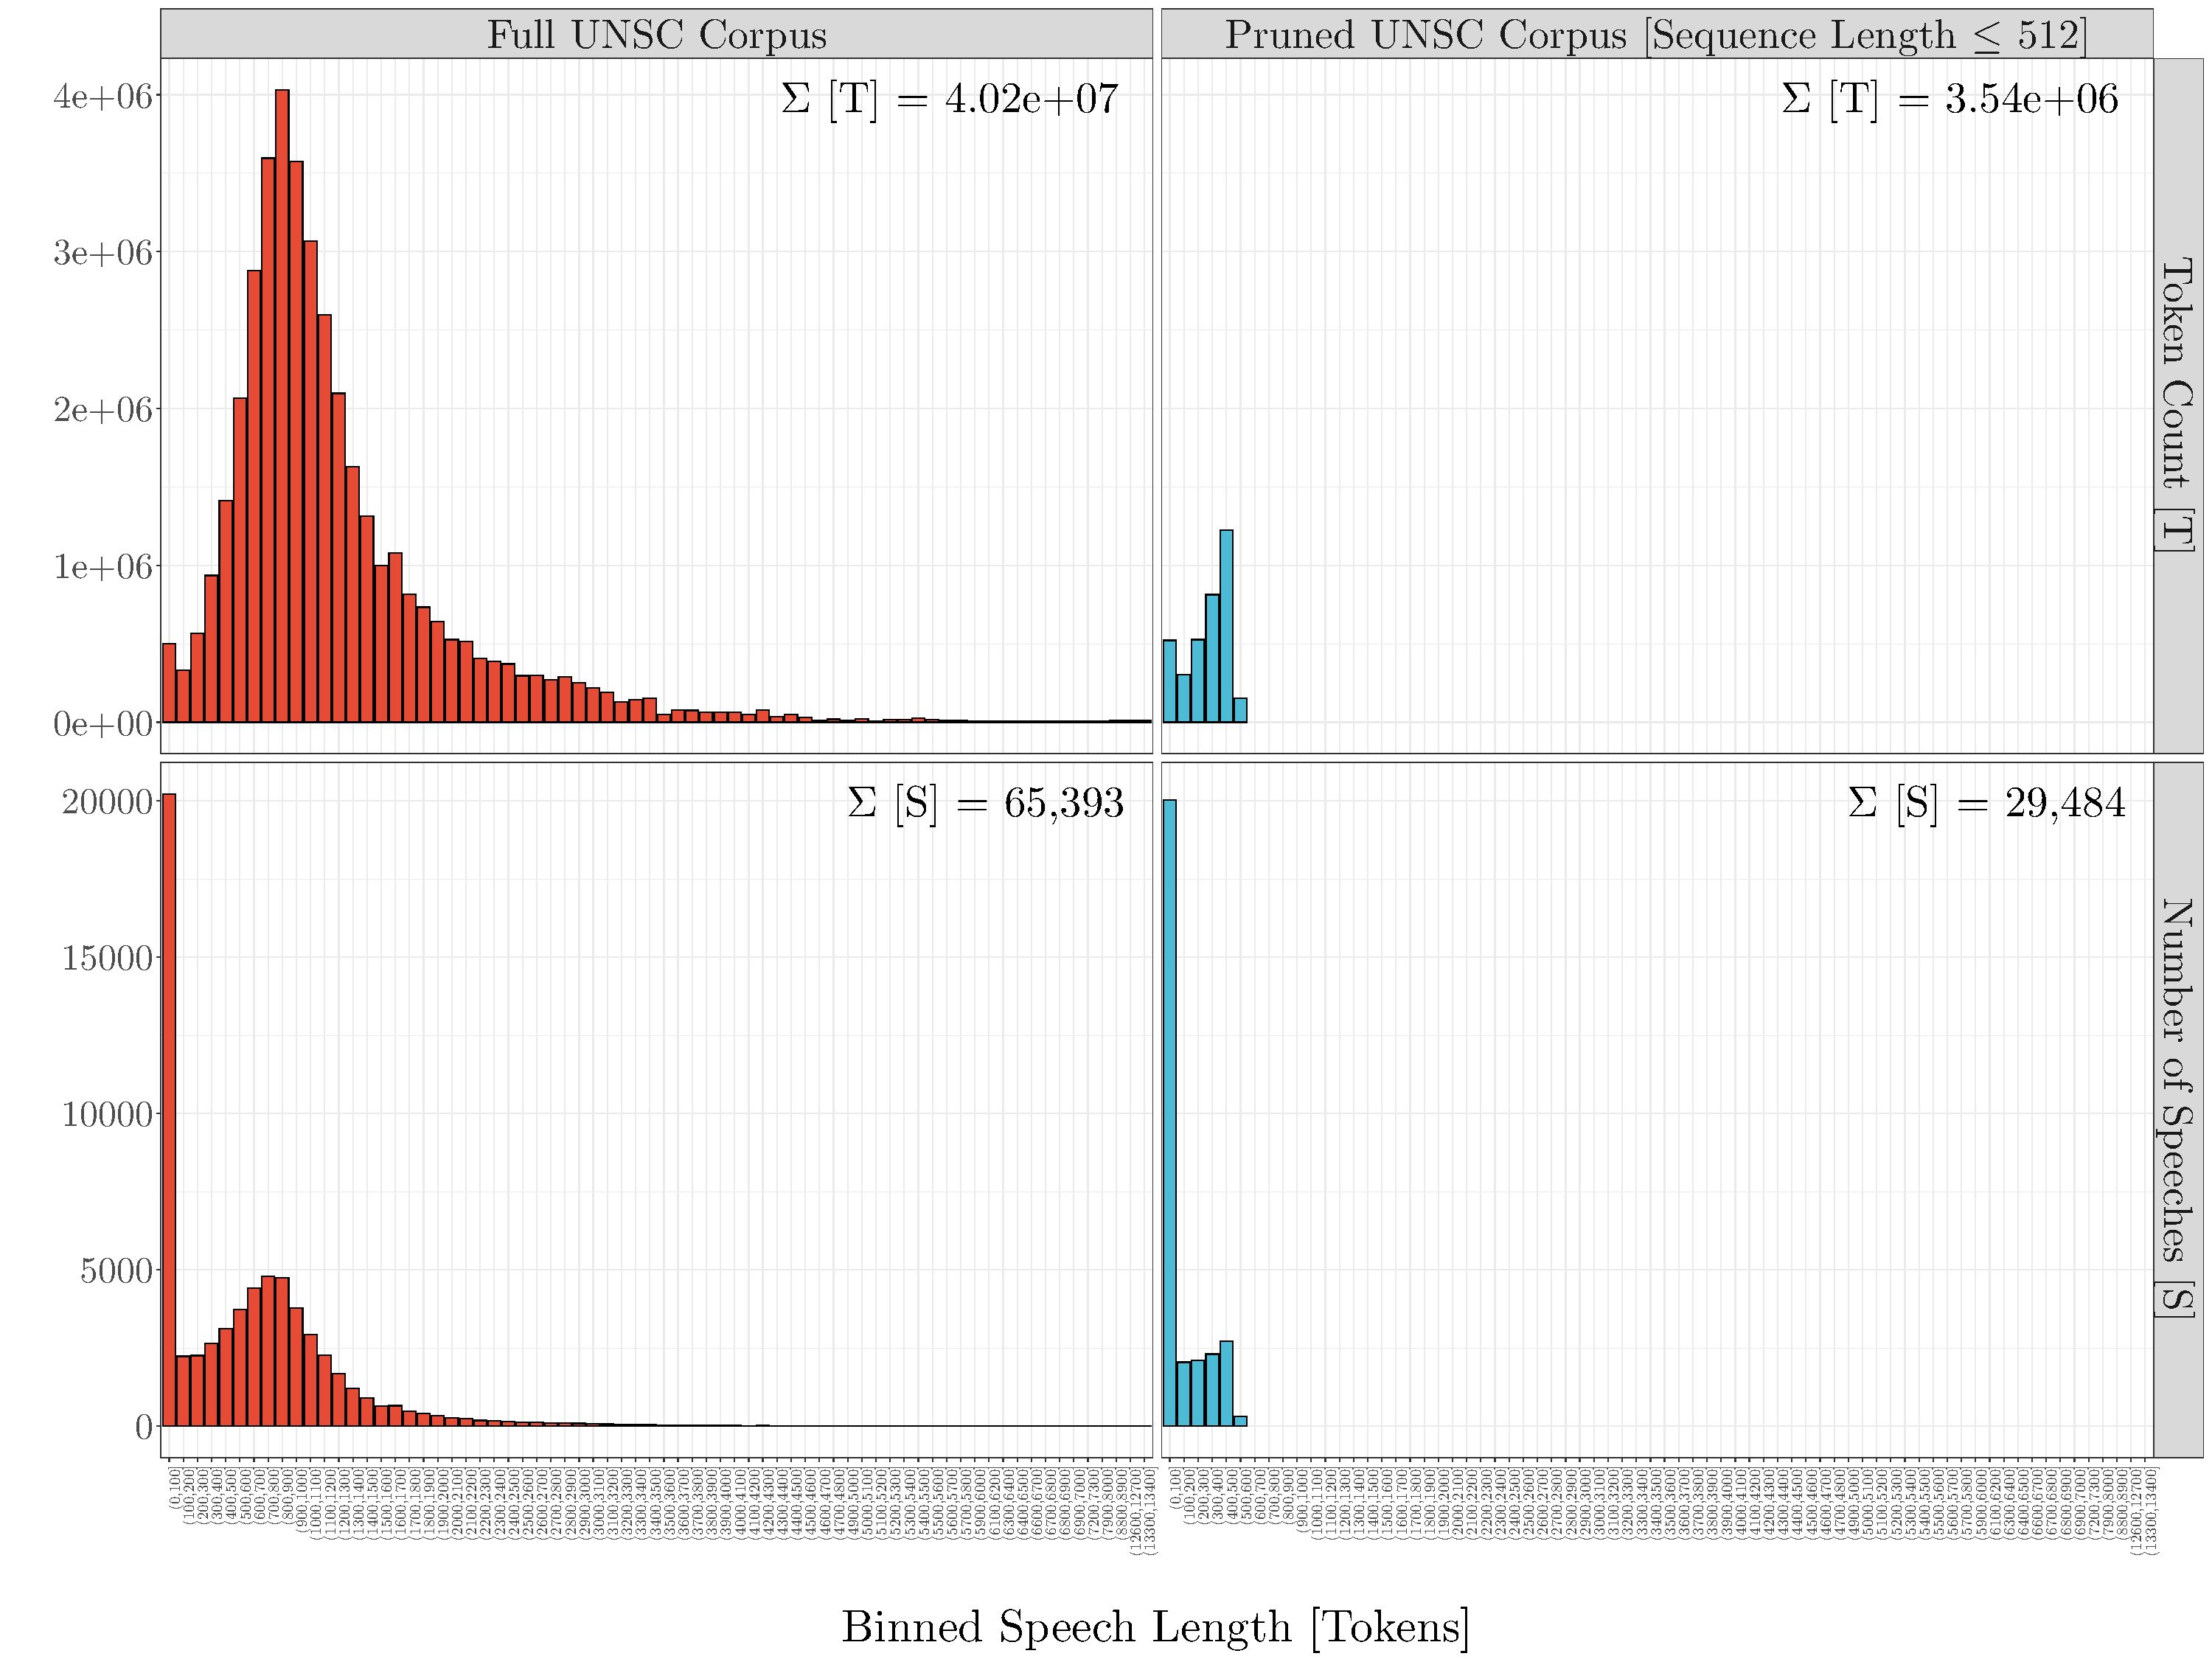
\includegraphics[trim={1.0cm 0cm 0cm 0cm},clip,width=\textwidth]{img/token_dist_UNSC_length_combined.pdf}
    \caption{Full UNSC corpus (left-column) and pruned UNSC corpus (right-column) by binned speech length with token count (top-row) and number of speeches (bottom-row)}
    \label{unsc_distribution_combined}
\end{figure}

Following a similar approach from \citet{eger2017neural}, we start by preparing the USED corpus for a sequence tagging task. Firstly, we converted character span annotations in the USED corpus to token-level annotations. Each token in the USED corpus gets mapped to one of three labels; specifically the ``None" (N), ``Claim" (C) or ``Premise" (P) label. Speeches that had at least one of either C or P tokens are considered argumentative (A), while speeches containing only N tokens are considered non-argumentative (O). The left column of Figure \ref{used_distribution_combined} shows the distribution of these classes of tokens as well as the number of speeches/types in the full USED corpus. It is worth noting that we omit the Beginning-Inside-Outside (BIO) tagging scheme as recommended in \citet{eger2017neural}; to keep our methodology simple and prevent label imbalances in the already small USED corpus. We also observe that sequences longer than 100 tokens tend to be more argumentative or have more C and P labels, indicating that longer sequences are of greater interest for argumentation mining in the USED corpus.

After mapping tokens to the aforementioned argumentation classes, we attempt to remove USED corpus-specific bias. In particular, we remove the initial token(s) in each speech where the identity of the person giving the speech is stated. Next, we use the SPM model to segment words into lowercased subwords; in accordance with the pre-packaged uncased ALBERT tokenizer. Finally we add BERT's special tokens; specifically a \texttt{[CLS]} and \texttt{[SEP]} token at the start and end of the sequence respectively. As mentioned in \ref{bert}, this process increases the token lengths of speeches; with some speeches exceeding the maximum sequence length of 512 tokens. To address this, we prune the USED corpus and remove sequences longer than 512 tokens. The effect of this pruning process can be seen in the right column of Figure \ref{used_distribution_combined}, with a minimal loss of 11$\%$ of tokens and 2$\%$ of speeches in the USED corpus.

The same data preprocessing procedure (naturally minus argumentation labelling) is then performed on the UNSC corpus to ensure that both these corpora can be treated similarly by the argumentation classifier model. For domain debiasing in the UNSC corpus, we also remove initial tokens which state the identity of the speaker. Figure \ref{unsc_distribution_combined} shows the effect of pruning on the UNSC corpus, with a much greater loss of 91$\%$ of tokens and 55$\%$ of speeches. Unfortunately, this is a necessary measure and is one of the major limitations of using the ALBERT model for such long sequences.

Finally, after pruning the corpora and having a clean set of input sequences, we insert BERT's \texttt{<pad>} tokens to cap up all sequences to 512 tokens, as this is necessary for the static computation graph that was implemented in our code. For evaluation purposes, we randomly split the USED corpus into \{training $\cup$ validation\} and test sets with a 70:30 ratio. We then split the \{training $\cup$ validation\} set into training and validation sets with a 85:15 ratio.

\subsubsection{Model Fine-Tuning and Evaluation}
\label{fine_tune}

\begin{table}[b]
	\centering
	\small
	\setlength{\tabcolsep}{0.5em}
	\def\arraystretch{1.1}
	\begin{threeparttable}
		\begin{tabular}{L{0.19\linewidth} p{0.52\linewidth} L{0.01\linewidth} L{0.17\linewidth}}
			\toprule[0.25mm]
			Model & Description && Parameters \\
			\midrule[0.35mm]
			TD$\_$Dense & 5 stacked time-distributed dense layers on top of the ALBERT model; with Rectified Linear Unit (ReLU) and softmax activations && 11,659,334 \\\\[-5pt]
			1D$\_$CNN & 5 stacked 1-dimensional convolutional layers on top of the ALBERT model; with ReLU and softmax activations && 12,790,598 \\\\[-5pt]
			Stacked$\_$LSTM & 3 stacked Long Short-Term Memory (LSTM) layers on top of the ALBERT model; with ReLU and softmax activations && 14,709,446 \\
			\bottomrule[0.25mm]
		\end{tabular}
		\caption{Tabular summary of three end-to-end ALBERT model types with custom decoders}
		\label{table_arg_train_models}
	\end{threeparttable}
\end{table}

As mentioned in section \ref{albert}, we decided that the ALBERT language model would be a good choice for us to fine-tune for our argumentation mining task. With the USED and UNSC corpora preprocessed, we needed to finalize the ALBERT model for fine-tuning. Out of the box, the ALBERT model is an encoder model. In order to use it for a supervised argumentation sequence tagging task, we would need to extend ALBERT with custom decoders such that the output of the model would be in the appropriate dimensions. Table \ref{table_arg_train_models} provides a summary of three models that we fine-tuned in this study.

For the fine-tuning process, we assume a warmup-cooldown learning rate profile, where the learning rate rises linearly over the warmup epochs until a maximum learning rate and then exponentially decays till an end learning rate at a fixed upper limit of 100 epochs. We utilize the Adam optimizer for fine-tuning all our models. To determine the best model and corresponding hyperparameters, we conduct a grid-search over model-type, warmup-epochs, maximum learning rate and end learning rate.

It is worth noting here that we fix our fine-tuning batch-size at 10 samples to prevent GPU out-of-memory (OOM) issues. This is mainly because the ALBERT model has a high memory consumption that is exacerbated by its $O(N^2)$ space complexity due to the self-attention mechanism, where $N$ is the input sequence length. Because of this, our model fine-tuning process suffers from noisy gradients. We recommend solutions for this issue in section \ref{reco} of our study.

For the evaluation process, we employ early stopping with a patience value of 5 epochs; measuring the cross-entropy loss on the validation set. At the end of fine-tuning each model, we compute the model's performance on the test dataset and record its Macro-F$_1$ score over N, C and P argument labels. The model with the best test F$_1$ score is deemed as the best performing model. We provide our best fine-tuned model in our GitHub repository\footnotemark[\value{footnote}].

For all the aforementioned processes, we utilized the \texttt{bert-for-tf2} python library, which is written using Google's \texttt{TensorFlow} API. In terms of hardware, we utilized a single NVIDIA GeForce GTX 1080 Ti GPU with 12 GB RAM provided by the University of Potsdam.

\subsubsection{Prediction on UNSC}

After following the aforementioned fine-tuning and model evaluation process, we arrive at our best performing model. In order to use this model to predict argumentation token-level argumentation candidates in the UNSC corpus, we simply pipe the preprocessed UNSC corpus into the model and acquire the model's outputs.

Due to the static configuration of our model, the output will have a sequence length of 512 tokens. We then remove the output sequence positons which correspond to the BERT \texttt{[CLS]}, \texttt{[SEP]} and \texttt{<pad>} special tokens; leaving behind only the important sub-word tokens that have been classified into N, C or P argumentation candidates. As a final product, we compile our UNSC predictions into a human-readable \texttt{json} file in our GitHub repository\footnotemark[\value{footnote}], which maps UNSC speech IDs to token-level argumentation predictions.